\section{Analyse à gros grain}
\label{sec:analyse_gros_grain}

\subsection{Première experience}

\subsection{deuxième expérience}

\subsubsection{Métriques et Renommage}
Un gestionnaire de versions (VCS) offre plusieurs moyens de calculer ces métriques car il stocke les informations sur les entités modifiés à chaque nouvelle version, l'auteur de ces modifications, la date etc. De plus il permet la récupération du contenu de chaque entité et de l'ensemble d'un projet à une version donnée. Pour calculer ces métriques, il est donc possible d'analyser chaque entités modifiés lors d'une période puis de ne garder uniquement les entités toujours présente à la dernière version de notre période.\\
Par ailleurs, il faut noter qu'un VCS identifie une entité par son chemin + nom de fichier. On en déduit qu'un renommage du fichier ou d'un dossier, aura un impact sur le calcul des métriques. Pour expliquer cet impact, on présente un exemple d'historique d'un logiciel figure 1. Ce projet ne contient qu'une entité, Test.php, qui est renommé en Hello.php dans la dernière version. Dans cet exemple nous calculons NoD entre la version 1 et 3.\\
Le NoD d'un entité de code source au cours d'une période de son histoire correspond au nombre de développeurs ayant étés identifiés comme auteurs d'une modification sur l'entité pendant la période donnée.\\

\begin{figure}[t]
	\centering
	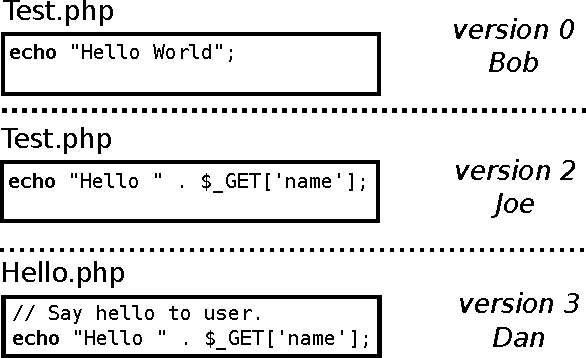
\includegraphics[width=0.8\linewidth,keepaspectratio]{data/figures/example.pdf}
	\caption{Example of a project history. The project is composed of only one file \texttt{Test.php} which is renamed to \texttt{Hello.php} in the last version.}
	\label{fig:example}
\end{figure}

La dernière version ne contient qu'une entité. C'est donc cette entité uniquement qui sera considérée. De plus l'identité exacte de cette entité n'aparait que lors de la version 3. Le calcul des métriques est donc trivial, NoD = 1, NoC = 1, CC = 2.\\
Par ailleurs, si on prend en compte le fait que ce fichié a été renommé, il y a trois versions à regarder en ce qui concerne l'entité. etc...TODO\\

Nous avons choisi de nous concentrer sur les trois métriques de procédés identifiés plus tôt pour mesurer l'impact du renommage. A partir de script Ruby sur nos projets, voici plus précisement comment nous avons procédés pour les calculer: (TOTO)\\
NOD:\\
NOC:\\
CC:\\ 
